\chapter{Módelos Bioeléctricos}

\begin{resumen}
  En esta sección se abarcan los conceptos básicos de anatomía y fisiología
  cardiaca, dando un repaso por las arritmias cardiacas, en especial la
  fibrilación. Luego se pasa a los módelos matemáticos que describen la
  actividad electrica de la células y el tejido  cardiaco en 2D y 3D realistas.
  A posteriori se analizan los diferentes módelos para la generación y
  propagación de la actividad eléctrica del miocardio. Se hace una descripción
  y análisis del módelo \ac{AC} propuesto en \cite{Alonso-Atienza05},  como un
  módelo de baja carga computacional. Se presenta el módelo \ac{LRd}
  \cite{luo1994, livshitz2007}, módelo celular cardiaco que representar el
  comportamiento de las corrientes ionicas de las células ventriculares. Para
  concluir el capitulo, se hace una introducción a los sistema de medida
  simulados, en donde se plantea la definicion de \ac{MSD}, usada a posteriori
  para el cálculo de volumen equivalente. Está da un acercando a la simulación cardiacas que se trabaja en esta Tesis.


 \TODO{hablar de velocidad de conducción que sera usada en el autómata
  celular}

\commentDir{ ... }

\end{resumen}


\section{Introducción}

% La contracción coordinada del corazón es resposable del eficaz bombeo de la
% sangre a travez del sistema cardiovascular. Esta coordinación se realiza
% mediante el sistema de conducción eléctrica del corazón, que controla el tiempo
% exacto en el que se realiza la contracción del miocardio a traves de un sistema de
% estimulación intrinsico, el cual fija la tasa de bombeo del sistema
% cardiovascular. El sistema de estimulos es espontaneo y de manera regular mandas
% los impulsos eléctricos, el cual se distribuye, gracias a sistema especializado
% de conducción, a través de todas las celular del corazón. Es asi como un sistema
% electro-mécanico de excitación-cotracción ocasiona el bombeo sistemático de la
% sangre, y a lo que en situaciones nornales se le denimina ciclo cardiaco,
% periodo donde el corazón alterna entre una contracción y una relajación.
%
%
% Cuando se presentan alguna alteración en el ciclo cardiaco, bien sea por
% alteraciones en la generación y/o en la conducción de los impulsos eléctricos,
% se habla de transtornos cardiacos, conocidos como arritmias. Las arritmias de
% mayor estudio, ya que su comprensión sigo siendo algo difusa, es la \acf{VF} y
% la \acf{AF}. La fibrilación en un contracción asincrónica y desordenada del
% tejido cardiaco. La \ac{AF} es la arritmia mas frecuente y aunque no es letal,
% si conlleva a enfermedades crónicas, su tratamientos puede llegar a la ablación
% con catéter de radio frecuencia.  Para enterder los mecanismos que dan lugar
% a las \ac{VF} y \ac{AF}, en la literatura se expone un conjunto de modelos
% electrofisiológicos y de técnicas de procesado de señal, los cuales permiten
% analizar el comportamiento del sustrato cardiaco con distintas patológias.
%
%
% Por su parte, el registro de la actividad eléctrica, en un ambiente clinico se
% realiza mediante sistemas de electrodos intracardiacos \ac{EGM}, que registran
% la actividad local del corazón, o en la superficie del corazón \ac{ECG}, que
% proporcionan una visión global del ciclo cardiaco. en un ambiente experimental
%
%
%

\subsection{Anatomía y fisiología de las celular}

% La anatomía del corazón se puede describir desde un  mirada espacial. De manera,
% macroscopia, la descripción espacial del corazon humano, indica que el corazón
% se encuentra al interior del tórax y contiguo a los pulmones. El musculo
% cardiaco se encuentra recubierto por el saco pericárdiaco, y acorde con el
% sistema circulatorio su funcionamiento se divider dos secciones anatomicamente similiares, la mitad
% derecha e izquierda. A su estas dos mitadas, se dividen en dos cavidades. Las
% cavidades superiores, auriculas, se encargan de recibir la sangre, y las
% cavidades  inferiores, ventriculos,bombean la sangre al sitemas circulatorio.
%
% Por un lado, la estructura derecha del corazón, a través de la auricula derecha,
% recibe la sangre desoxigenda del cuerpo  y la bombea, desde el ventriculo
% derecho, a los pulmones. De forma paralela, la mitad izquierda del corazón
% recibe la sangre oxigenada, en la aurícula izquierda, proveniente de los
% pulmones, y a posteriori, por medio del ventriculo izquierdo, abastecer a todo
% el cuerpo incluido el propio corazón con la sangre ya oxigenada.
% El ventriculo izquierdo, tiene una cavidad mucho
% más gruesa y fuerte que su homologo derecho.
%
% Desde una mirada anatómica, las cuatro cavidades del corazón, 2 aurículas y
% dos ventíiculos, estan compuestas de un músculo estructural denominado
% miocardio. El miocardio, esta cubierto el interior de las cavidades por el
% tejido endocardiaco. Al exterior de las pared miocardiaca se encuentra el tejido
% epicardiaco. A si mismo, se habla que el miocardio esta dividido en
% pared subepicárdica, pared media y pared subendocárdica. El flujo de sangre
% entre auriculas y ventriculos, es controlado por las válvulas tricúspide  y la
% mitral, ubicadas en la la estructura derecha e izquierda respectivamente.
% La válvula pulmonar controla el flujo sanguíneo del ventrículo derecho a las
% arterias pulmonares y la válvula aórtica controla el paso de la sangre oxigenada
% desde el ventrículo izquierdo a la aorta.
%
% En resumen, la función del corazón es proveer al todo el cuerpo la sangre
% oxigenada, y para ello, el corazon ejecuta tres movimientos autónomos que le
% permite bombear la sangre al cuerpo, sístole auricular y ventricular y  la
% diástole, movimientos de contracción y dilatación respectivamente. la generación
% de estos eventos cardiacos, el músculo cardiaco se autoestimula y la secuencia
% de las contracciones cardiacas son producida  por la despolarización de las
% células cardiacas, y  propagada por el miocardio, a través del sistema de
% conducción del corazón.
%
%
\subsubsection{Actividad eléctrica del corazón }

% El origen de la actividad eléctrica del corazón son los miocitos. La actividad
% eléctrica de cada miocito del corazón, genera cambios transitorios en el
% potencial de menbrana, \ac{AP}. El \ac{AP} es el producto de la actividad
% electroquimica que genera el intercambio de iones, a través de los canales
% iónicos  y bombas elctrogénicas, en la membrana células. Estos intercambios
% generan impulsos eléctricos que se propagan a través del tejido. En las células
% cardiacas, los impulso eléctrico genera la contracción sincronizada de todas
% las células  que están eléctricamente acopladas, trayendo consigo que todas las
% cámaras en el corazón se contraigan.
%
% Por lo tanto, hablamos de exítabilidad, cuado a un estímulo suficientemente
% fuertes se presenta un cambio transitorio de la polaridad del voltaje
% transmembrana. De esta manera, se entiendo que cada célula cardiaca tiene
% asociado un proceso de contracción asociado a su \ac{AP} respectivo. en el
% \ac{AP} de cada célula se distinguen dos estados, cuando la célula esta en
% reposo o cuando esta en estado activo.
%
% Con la menbrana en estado en reposo, la célula está en equilibrio dinámico el
% medio intracelular está a menor potencial que el extracelular. La membrana es
%  ligueramente impermeable al sodio (Na+) y un poco permeable al potacio  (K+) y
%  al calcio (ca 2+). En respuesta a un estímulo eléctrico o mecánico, la
%  permeabilidad de la membrana se modifica, lo que conlleva a que los iones de
%  potasio puedan salir de la célula de una forma más eficiente de lo que pueden
%  llegar a entrar los iones de sodio, que provoca la despolarización celular, es
%  decir, un cambio en el potencial eléctrico transmembrana. cuando la célula esta
%  despolarizada se habla de esta manera de estado activo. Inmediatamente, el
%  equilibrio i onico tiende a restablecerse de forma progresiva durante el
%  proceso denominado repolarización.
%  La membranas células excitables, de esta manera, tienen la capacidad de
%  modificar la polaridad ante estímulos, que superen el umbral de activación, y
%  generar un \ac{AP}, gracias a la diferencia de concentraciones iónicas entre
%  los dos medios, y por lo tanto, entre las fuerzas de difusión  y de campo eléctrico.
%
% El \ac{AP} caracteriza, en parte, la propagacíon de la despolarización del
% tejido cardiaco. Es asi como, el tiempo entre de pasar de estado de reposo a
% estado activo  y retornar al estado de reposo, se le da el nombre de
% \ac{APD}. En  la \ref{fig:apds} se observan diferentes \ac{APD} y esto es porque
% el corazón esta formado por distintos tipos de celular cardiacas y por lo
% tanto, presentan distintas formas de \ac{AP}, \cite{dawodu1996, Malmivuo95,
% Sachse04}.
%
%
%
% \begin{figure}[t]
% \centering
%  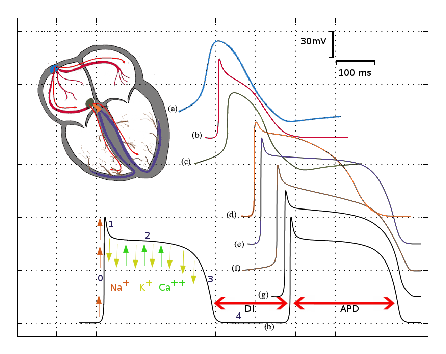
\epsfig{file = ./images/01_chap/APDs2.eps,width = 15cm}
% \caption{Cambio transitorio del voltaje transmembrana, durante un potencial de
% acción:(a) Nodo sinusal, (b) Auricula, (c) Nodo Auriculo-ventricular (d)
% His-bundle,  (e) His-Tawara, (f) Fibras de Purkinje, (g)
% Ventriculo (Subendocárdico), (h) Ventriculo (subepicárdico). }
%   \label{fig:apds}
% \end{figure}
%
%
% Como se observa en \ref{fig:apds}(h), el \ac{AP} de los ventriculos  presentan
% cinco fases distintas, esta caracterización fisiológico comprende:
%
% La fase ascendente del \ac{AP}, es el cambio drástico del potencial inicial de
% la menbra. En esta fase, conocida como fase 0, la membrana,  de forma
% abrupta, permite el ingreso masivo de iones de sodio ($Na^+$) por unos cuantos
% segundos.
%
% La  fase de repolarización inicial, es el instante en que los canales de sodios
% se inactivan, y se abren los canales de potasio ($K^+$). En esta fase 1, se
% provocando asi una pequeña repolarización rapida del \ac{AP}, debido a las corrientes de
% salida de potasio.
%
% En la siguiente fase, el \ac{AP} se mantiene casi constante (cercano a los
% 0mV), y se conoce como fase de meseta o fase 2. En esta fase se activan los
% canales de Calcio $(Ca^{2+}$). en esta fase las corrientes de calcio
% son compensadas por las corrientes de potacio, generando el efecto meseta del
% \ac{AP}.
%
% En la fase 3, se inactivan los canales de calcio, y sólo los canales de
% potasio quedan activos, permitiendo que el procesos de polarizacion se
% accelere. a esta fase se le conoce como fase repolarización final.
%
% Por último la el \ac{AP} en estado de reposo, entra a la fase 4, y el potencia
% de la menbrana, estable y constante, queda a la espera de un nuevo estimulo que
% supere el potencial de umbral, para generar un nuevo \ac{AP}. Al tiempo de
% recuperación, que va desde el final del \ac{APD}, hasta el comienzo de un nuevo
% \ac{APD}, se loe conoce como \ac{DI}.
%
%
% El músculo cardíaco, en condiciones normales, se contrae de acuerdo con los
% impulso generados por celular autoexitables, ubicados en algunas zonas del corazon. Dos
% nodos autoexitables, que se presentan en la \ref{fig:apds}(a) y (b), son lo
% nodo sinusal y el nodo auriculo-ventricular, respectivamente. Estos dos nodos
% tienen la propiedad de despolarizarse de manera espontánea, es decir no es
% necesario la intervención de un estímulo externos. la \ref{fig:apds}(a) y (b)
% refleja como la membrana celular, de dichos nodos,  se despolariza lentamente
% durante la fase de reposo debido,principalmente, al cierre gradual de los
% canales de potasio y a que la entrada masiva de sodio en el interior de la
% célula no es tan rápida como en las celular del ventriculo. Al llegar al
% potencial umbral, se da inicio a la despolarización. en estos nodos se evidencia
% la ausencias de la fase de reposo, vista en el \ac{APD} de las células ventriculares.
%
%
% Las células cardiacas tiene la propiedad de excitabilidad, funcion de \ac{APD}
% y del \ac{DI}, y que, en la mayorias de las células del corazón, es
% consecuencia de un estimula externos. Pero esta propiedad  de excitabilidad, no
% se cumple, por un periodo dentro del tiempo \ac{AP}. El tiempo refractario, o
% fase de refractariedad, como se le denomina a este periodo de no exitabilidad,
% es el tiempo en el que la celular exitable no responde a un estimula externo,
% sin importar su intensidad.
%
% Por consiguiente, al variar la frecuencia de estimulación del corazon
% varia el \ac{DI}. Se estima que el tiempo refractario sea
% mayor cuando \ac{DI} es mayor, y viceversa. En consecuencia,
% el \ac{APD}, es función tanto del \ac{DI}, como del \ac{APD} predecesor.  El
% \ac{APD} dismunuye con la disminución del \ac{DI} y con el incremento en la
% frecuencia de estimulación. La relación entre \ac{APD} y \ac{DI} se conoce como
% curva de restitución, y se observa en \ref{fig:curvares}.
%
% \begin{figure}[t]
% \centering
%  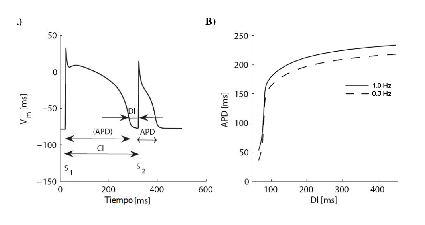
\epsfig{file = ./images/01_chap/curvarestitucion.eps,width = 15cm}
% \caption{Cambio esta curva  esta es vil copia del libro }
%   \label{fig:curvares}
% \end{figure}
%
\subsubsection{Sistema de propagación}

% El músculo cardiaco esta conformado por miocitos y por fibras
% musculares. Los miocitos que componen una fibra muscular está conectados en
% serie entre sí, y favorecen la propagación del impulso eléctrico en la
% dirección del eje de la fibra muscular. La despolarización en un miocito, genera
% a su vez estímulos eléctricos que despolarizan otras celularas vecinas interconectadas electrícamente.
%
% La principal propiedad del tejido cardiaca  es la propagación del \ac{AP}.
% Durrer junto con sus colaboradores en \cite{durrer1970}, presentan el estudio de
% la velocidad de propagación del corazón humano aislado. Cuando una célula es
% estimulada, es decir  inicia la despolarización, la diferencia de potencial
% intracelular, aumenta. y por lo tanto, se genera una corriente eléctrica, entre
% la célula recien despolarizada  y las célula contigua, lo que conlleva al
% aumento del potencial interto de la celular vecina. cuando el potencial interno
% de la célula vecina,  supera el umbrar de desporalización, dicha celular se
% exita. Este proceso se repite con la nueva célula, lo que conlleva a la
% propagación del \ac{AP} \cite{jalife2011}.
%
% Para la propagación ordenada, en
% condiciones normales de un ciclo cardíaco, el \ac{AP} es iniciado en el nodo
% sinusal, poropagandose por la auriculas. Estas a su vez, estan separadas
% electricante  de los ventriculos, y por lo tanto, el \ac{AP} viaja por el nodo
% auriculo-ventricular, que conecta eléctricante las auriculos  con los
% ventriculos. El nodo auriculo-ventricular actúan como línea de retardo para
% lograr una temporización adecuada entre la acción de las aurículas y
% ventrículo. Una vez terminada la contracción de la auriculas, el estimulo  se
% propaga desde el has de hiz al sistema de His-Purkinje, desde el cual el
% \ac{AP}  se distribuye por el resto de los miocitos  ventriculares. La velocidad
% de conducción del \ac{AP} depende, principalmente, de la dirección en la que se
% propaga. el sistema de propagación del \ac{AP} se observar en la parte superior
% izquierda de la \ref{fig:apds}, el cual se conoce como tejido especializado de
% conducción.
%
% Al igual que la dependencia del valor de \ac{APD} con respecto al \ac{DI},  la
% propagación del impuso es caracterizado por \acf{CV}. \ac{CV} tambien
% es dependiente de \ac{DI}. En la Figura XXX, se muestra la relación entre el
% \ac{CV} y el \ac{DI}. Como se puede observar, y al igual que en el \ac{APD}, la
% \ac{CV} disminuye cuando el \ac{DI} disminye, por lo tanto, se dice que a una
% tasa de activacion cardiaca mayor, la velocidad de propagacion del estímulo sera
% menor.
%

\section{Módelo Electrofisiológico} \label{sec:modelElectrofi}

% Por lo expuesto en la sección anterior, se evidencia la actividad
% electrofisiológica del corazón, puede ser  modelada bajos aproximaciones
% matematicas, que permiten hoy por hoy realizar estudios cardiacos, por medio de
% simulaciones de computador de las diversas dinamicas cardíacas. Desde un punto
% de vista matemático, podemos describir, tanto el flujo de corriente ionicas en
% los miocitos, como modelar el sistemas de propagación de \ac{AP}. Como se discution en el apartado
% anterior, el aspecto más importante de la dinamica del tejido es el \ac{AP}, y
% por lo tanto, los módelos  electrófisiológicos, principalmente, se basan  en la
% simulación del \ac{AP}. Es asi, como existen diversos módelos computacionales
% electrofisiológicos, que se clasifican acorde  a la complejidad asociada a la
% representaciòn del funcionamiento del miocardio. Algunos modelos, simulan con
% ecuaciones las corrientes ionicas que atreviesan la menbrana celular.
%
%
% Los módelos matematicos de la membrana celular, que describen el
% flujo de corrientes se basan, principalmente, en el
% trabajo desarrollado por Hodgkin-Huxley \cite{Hodgkin52}. este módelo se observa
% en la figura \ref{fig:circuitomembrana}. el módelo esta  basado en las curvas de corriente
% nedidas en unsa célula nerviosa, por lo cual no se evidencia la contribución de
% la corriente de Calcio, que presenta la excitación en los miocitos. en la figura
% \ref{fig:circuitomembrana}, se presenta las contribuciones de las corrientes
% generadas por el flujo de sodio ($I_{N_a}$), de potasio ($I_{k}$),  y otros
% iones ($I_L (leak current)$). Ademas,  $V_m$,  representa el potencial de
% membrana, definido como la diferencia entre los potenciales intracelular
% $\Phi_i$ y extracelular $\Phi_e$, por último $C_m$ refleja el efecto
% capacitivo de membrana. El módelo permite calcular las corrientes iónicas de
% diferente tipo que pasa a través de la membrana del axón y el voltaje de
% transmembrana. Asi el cambio  de $V_m$ en el tiempo se describe en
%  \ref{eq:N-N}:
%
% \begin{equation}\label{eq:N-N}
% \frac{\partial{\mathbf{V_m}}}{\partial{t}}=
% \frac{\partial{I_{m} - i_{stim}}}{\partial{C_m}}
% \end{equation}
%
% Donde, $I_m$ es la suma de las corriente iónicas que  atraviesan la
% membrana celular,$I_m = I_{Na} + I_K + I_l$ y y $I_{stim}$ representa la
% corriente de estimulación aplicada desde el medio extracelular.
%
%
% \begin{figure}[t]
% \centering
%  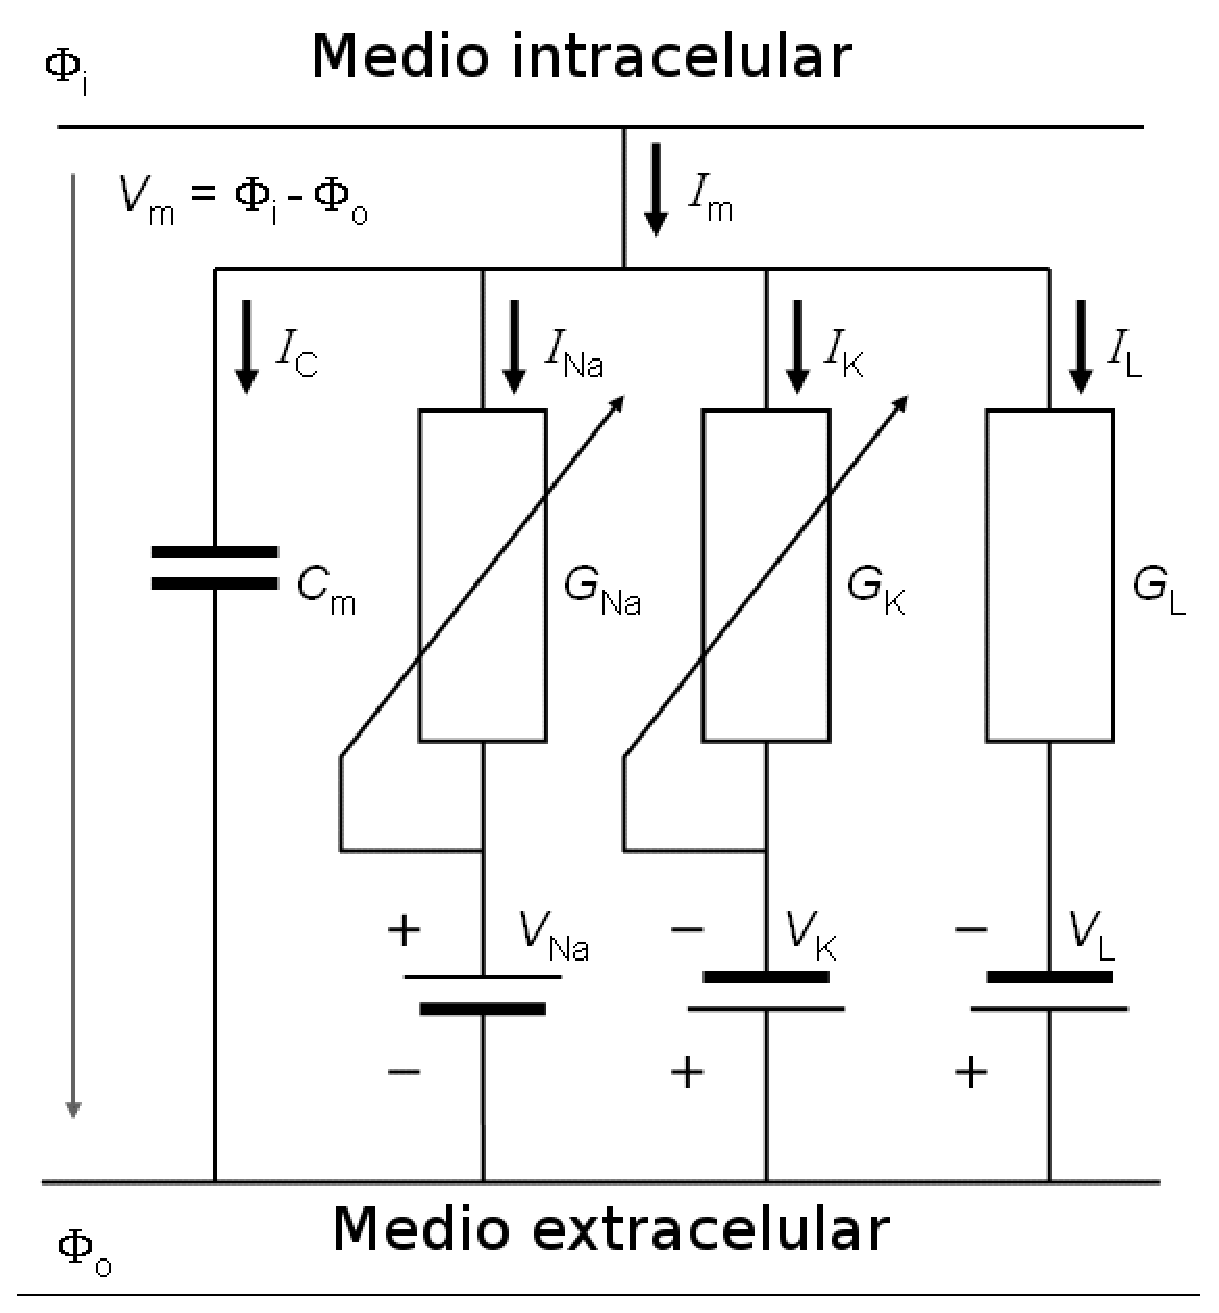
\epsfig{file = ./images/01_chap/circuitomembrana.eps,width = 8cm}
% \caption{Circuito equivalente de la membrana celular Hodgkin-Huxley }
%   \label{fig:circuitomembrana}
% \end{figure}
%
%
%
% \subsection{Módelo de la Célula}
%
% El módelo de Hodgkin-Huxley, se ha modificado por diversos
% autores, permitiendo simular miocitos de zonas especificas del tejido cardiaco,
% y con mayor complejida. En \cite{Sachse04}, se compila un listado de diversos
% autores, que han modelados los miocitos. Los primeros trabajos basados en
% el módelo de Hodgkin-Huxleym, y que dan inicio al módelo de células
% cardiacas, en especifico las fibras de purkinje, fueron los trabajo de Noble
% \cite{noble1962} y McAllister,R.E \cite{mcallister1975}.
%
% A posteriori, varios autores proponen diversos módelo del nodo sinusal en
% conejos \cite{noble1984, demir1994}. Por otra parte, las propuestas del módelo
% para los miocitos ventriculares, inician con le trabajo de Beeler y Reuter
% \cite{beeler1977}. El planteamiento mátematico de Beeler y Reutes, es
% replanteado en el trabajo de Luo y Rudy \cite{luo1991}. Este último módelo, con
% las respectivas actualzaciones  y revisiones \cite{luo1994, livshitz2007}, es
% posiblemente el mas utilizados hoy en día.
% Asi mismo en la literatura se encuentran varios autores que han módelado los
% ventriculos de maniferos, como conejos y perros \cite{courtemanche1998,
% demir1996, lindblad1996, noble1998}.  El desarrollo del módelo de la actividad
% electrica en venriculos humanos, en los  trabajos de
% \cite{nygren1998, bernus2002, sachse2003, ten2004}
%
% En los próximos dos apartados se presenta de manera resumida los
% dos módelos matemáticos, que son usados en esta Tesis: el módelo \acf{LRd} y el
% autómata celular. Ambos módelos nos permiten generar la actividad
% eléctrica en los miocitos y que posteriormente  son utilizados en la  simulación
% del tejidos cardiaco, para generar diversos tipos de arritmias, entre ella la
% fibrilación ventricular.
%
%

\subsection{Módelo Luo-Ruby}

% El módelo de \acf{LRd}, describe la electrofisiología de un miocito ventricular
% del cobayo. el módelos \ac{LRd}, espresa el formalísmo matematico del \ac{AP} a
% partir del desarrollo realizados por Beeler-Reuter \cite{beeler1977}, y aporta
% al módelo la contribción de que realza la concentración de calcio $Ca^{2+}$,
% en la despolarización de la celular, voltaje trasnmembrana. Desde publicacion
% incial \cite{luo1991}, y luego expandido en  \cite{luo1994}, se han tenido XX
% actualziaciones.  En \cite{zeng1995}, se separa la contribución de las
% corrientes de potasio, $I_{Kr}$ y $I_{Ks}$, en contribución rapida y lenta.
% a posterior se estudia los efectos de $I_{Kr}$ y $I_{Ks}$  en el \ac{APD}, dando
% como resultado la reformulación de la coriente $I_{Ks}$ acorde a tres tipos de
% células diferenten, epicardio, endocardio  y miocardio. este estudio se
% encuentra en \cite{viswanathan1999}. Un año mas tarde en \cite{faber2000} se
% incluye en el módelo el formalizmo matemático de la corriente generado por el intercambio de
% sodio-calcio. Asi mismo, Hund y Rudy en \cite{hund2004}, desarrolaron el
% formalismo matemático que modelar la electrofisiología de una célula ventricular
% del perro, \ac{HRd}.
%
%  Livshitz y  Rudy \cite{livshitz2007}  modifican los módelos \ac{LRd} y
%  \ac{HRd}, e incomporan nuevas relaciones entre el transiente de $Ca$, la
%  corriente $I_{ca_{(L)}}$. En resumen en la figura \ref{fig:modelHRd}, se
%  visualiza el actual módelo  \ac{LRd} de la celular cardiaca del ventriculo en
%  mamiferos,
%
%  Como se explico, en la anterior sección, hay un gran variedad de  módelos
%  cardiacos para diferentes mamiferos, donde se observan sutiles diferencias
%  elctrofisiológicas entre las especies, en relación a las corrientes y
%  canales ionicos. Entonces a distintos estimulos cada módelo cardiaco
%  tiene un comportamiento diferente, ya que la caracteristicas del \ac{AP}
%  varian entre cada especie \cite{OHara2012}, y son de  importnacia en el estudo
%  de respuesta a distintos fármacos. Sin embargo, esta pequeñas diferencias,
%  para efectos prácticos, en estudios donde trabaja a partir de las propiedades
%  macroscopias del \ac{AP} tiende a ser indiferente el tipo de módelo que sea
%  usado.
%
%   \begin{figure}[t]
% \centering
%  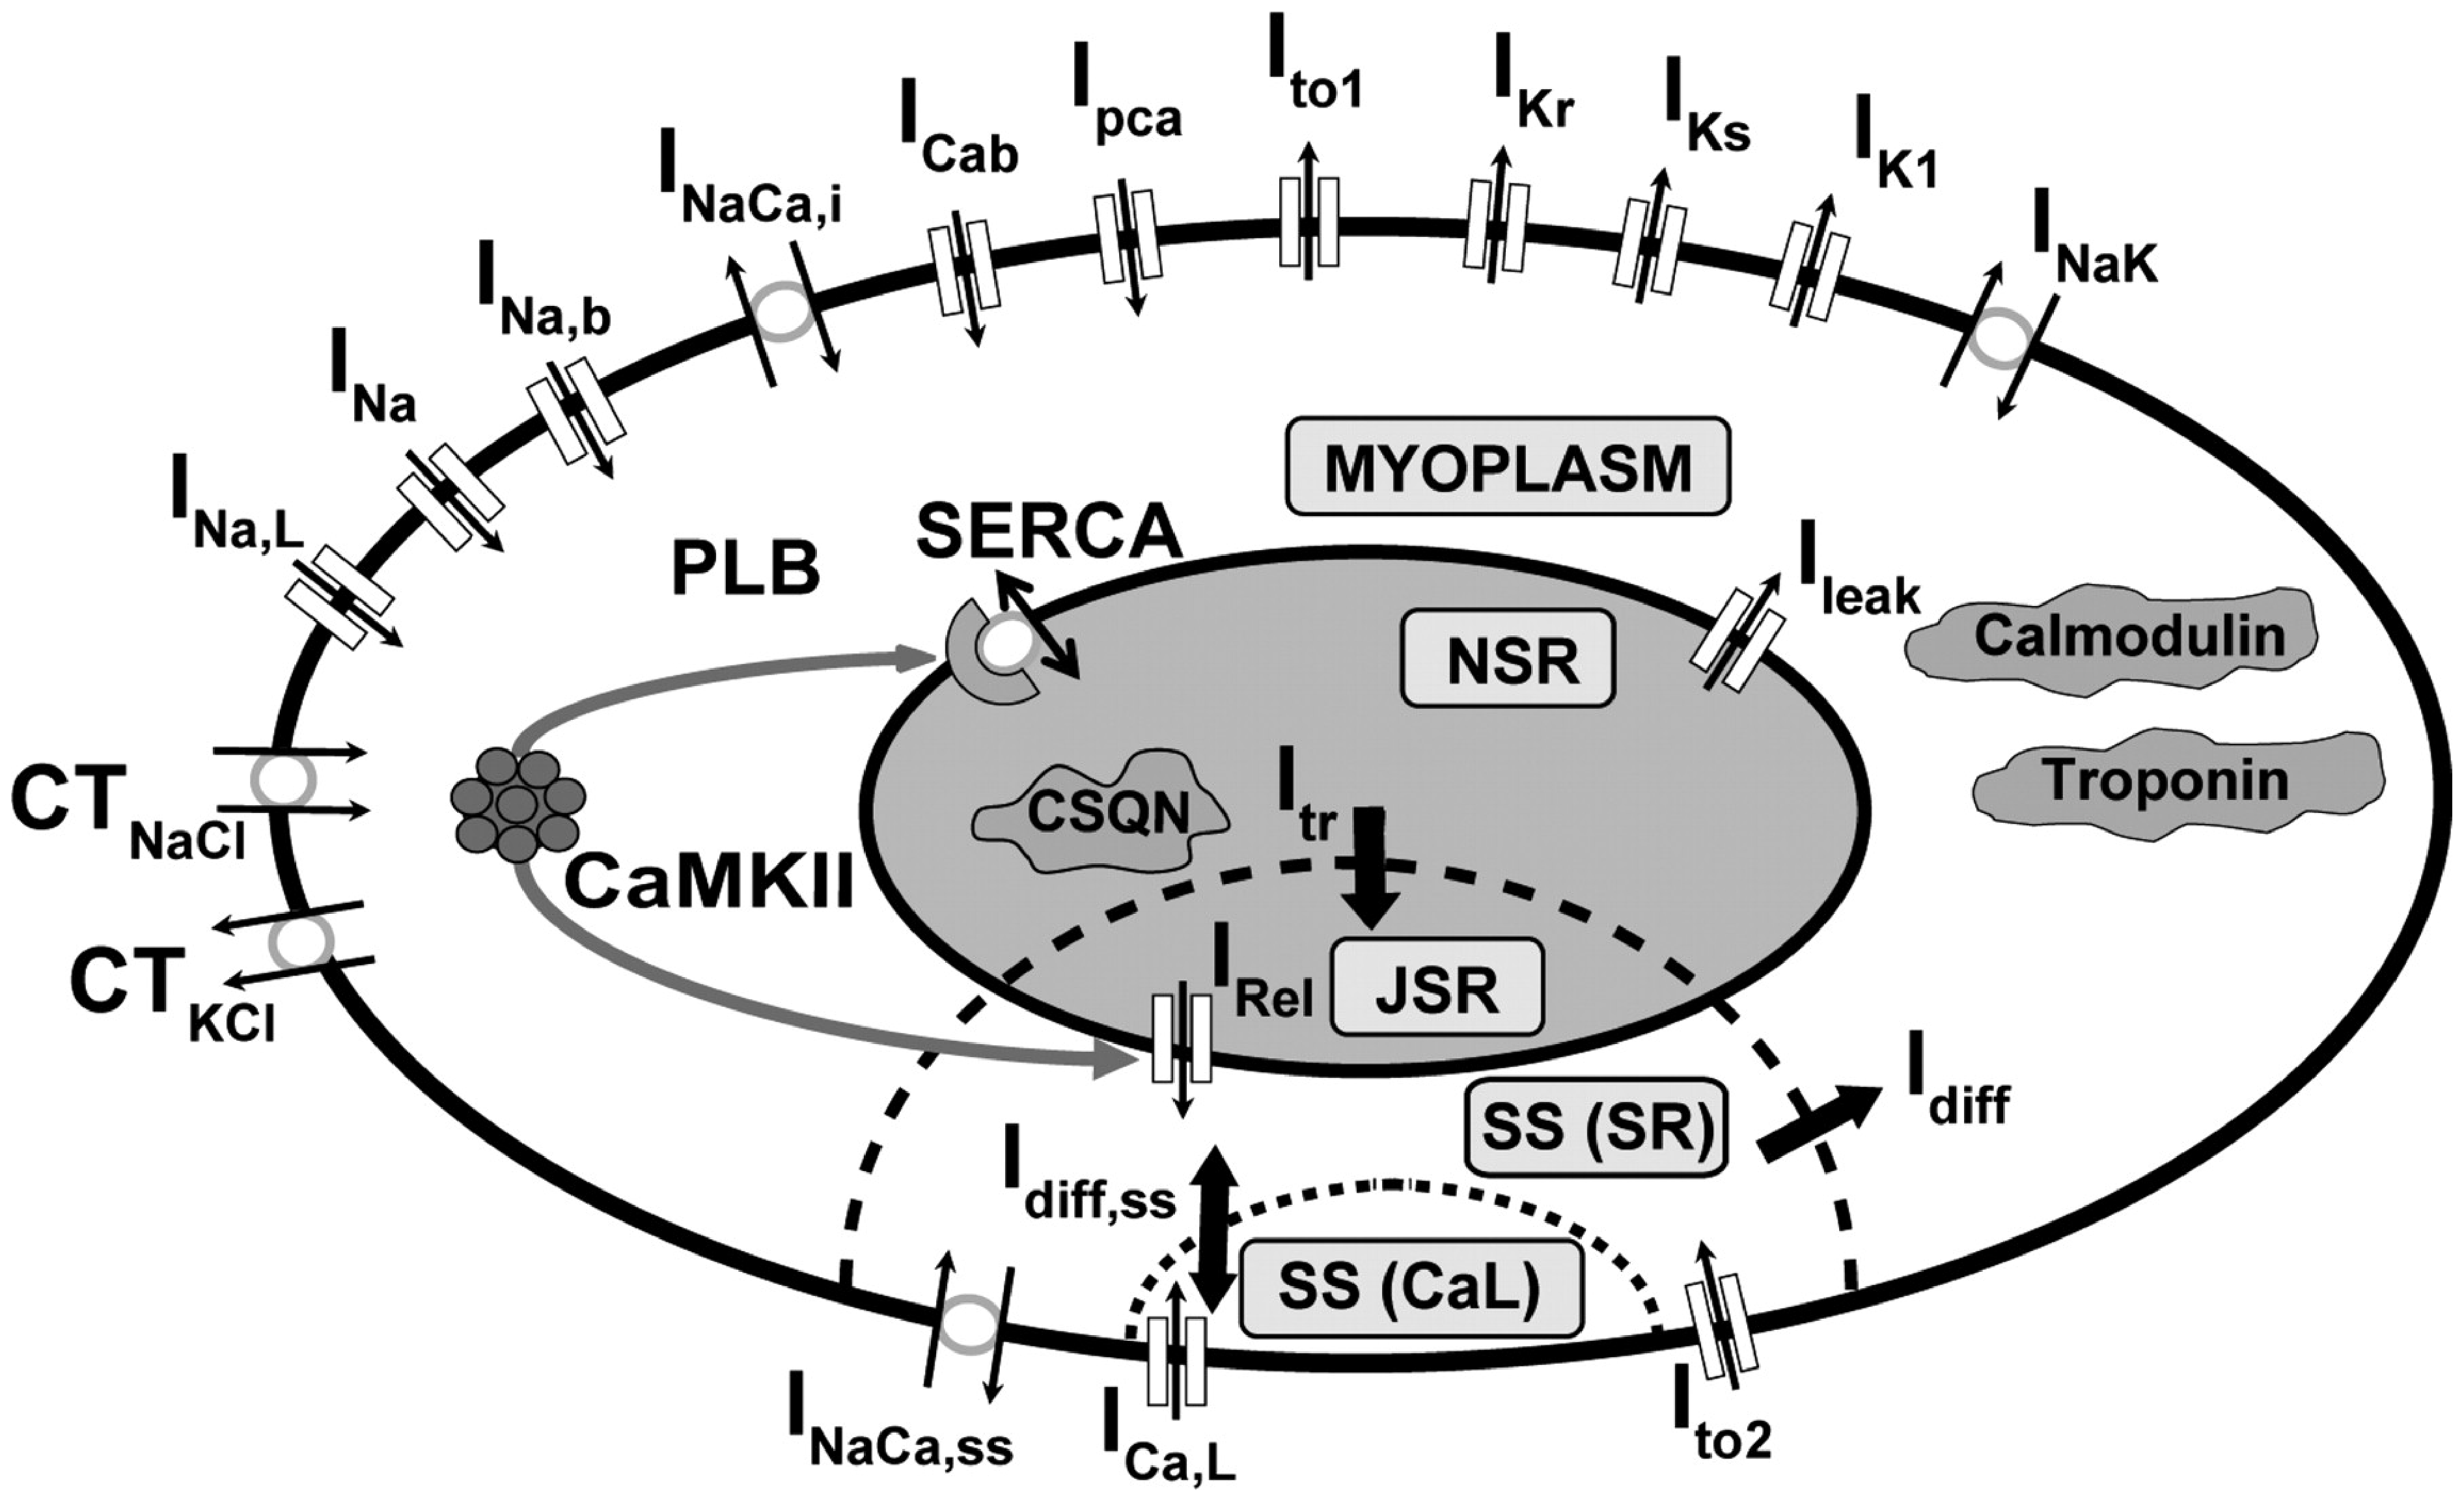
\epsfig{file = ./images/01_chap/modelHRd.eps,width = 10cm}
% \caption{bla bla ). tomado de la web de rudy }
%   \label{fig:modelHRd}
% \end{figure}
%
%
\subsection{Autómata Celular }

% Los autómatas celulares son ampliamente usados en diversas disciplinas. De igual
% maneras, en el contexto de cardiologia celular, un número bastante amplio de
% autores han modelado la actividad de la célula por medio del autómata celular.
% La ventaja de utilizar este sistema de \ac{AC}, es la eficiencia
% computacional que ofrece la versatilidad de variar las propiedades de conducción.
%
% Partiendo de la actividad eléctrica del miocito,  y principalmente de las
% caracteristicas del \ac{AP}, en el \ac{AC}propuesta en
% \cite{Alonso-Atienza05} la celular puede adopta 3 estados diferentes:
%
%
% \begin{itemize}
% \item Reposo: periodo  durante el cual la célula esta relaja  y puede ser
% estimulada por una fuente externa
% \item Refractario 1: la célula se encuentra excitada  y ademas tiene el
% suficiente potencial para excitar a células contiguas.
% \item Refractario 2: La célula se encuentra excitada, mas sin embargo, el nivel
% del \ac{AP} es bajo, y por lo cual pierde la capacidad de excitar a las células
% vecinas.
% \end{itemize}
%
% De esta manera, el periodo refractario 1 y 2 es el tiempo  en el cual la célula
% se encuentras despolarizada, y  por ende la despolarización del micito, sucede
% en la transición del estado de Reposo al estado Refractario 1. Por su parte, la
% fase 1 de repolalización parcial de \ac{AP}, debido a las corrientes de salida
% del potasio, corresponde a la transición del estado Refractario 1 al estado
% Refractario 2. La repolarización total de la célula, fase 2, se da en paso del
% estado Refractario 2 al estado de Reposo.
%
%
% La figura XXXX, muestra las caracteristicas del \ac{AP}. Asi mismo,las
% propiedades de restitución hacen que el \ac{APD} dependan directamente de la
% tasa de estimulación a la que este sometida la membrana celular. Al tener una
% frecuencia de estimulación elevada  se observa la reducción del \ac{DI}, y como causa, la
% reducción del \ac{APD}. Sucede lo contrario cuando el ritmo de excitación es
% bajo. De esta manera, en el \ac{AC} el tiempo es el estado en reposo es
% igual al \ac{DI} y para el \ac{APD}, se fija los tienpo de duración de los
% estados refractarios de manera fija, Es decir, el tiempo que permanece
% la célula es en estado Refractaio 1 es una fracción del tiempo total del
% \ac{APD}, por lo general el 10\%, y el restatan 90\% es, por lo tanto, el tiempo
% que dura la célula en el estado refractario 2. Es asi, como los tiempo de
% repolaización total y parcial se fijan acorde al valor de \ac{APD} predecesor.
%
% En cuanto a la despolarización del micito, en el autámata celular se da en
% función de la probabilidad de excitación de la célula cardiaca.
%
% falta la figura
%

\subsection{Módelo de Tejido}

% Por lo pronto se ha visto que los módelos computationales de miocitos cardíacos,
% han sido herramientas importantes para la comprensión del \ac{AP}. y por lo
% tanto, para entender los mecanismos que dan lugar a las diferentes arritmias
% cardiacas, se han modelados diversas aproximaciones que simulan la propagación
% del estímulo cardiaco. Al igual que los módelos de celular, los módelos de los
% tejidos cardiacos se agrupan en módelos microscopicos y macroscopicos.
%
% los módelos microscópicos del tejido del corazón, estan restringuidos a
% regiones pequeñas, debido la alta carga computacional que requiere al tener en
% cuenta un elevado numero de variables que contribuyen  tanto en el \ac{AP} como
% la velocidad de conducción.
%

\subsubsection{Módelo de la membrana en el autómata}

% El módelo \ac{AC} de la membrana esta conformado, como se observa en la Figura
% \ref{fig:automata1},  por la red discreta de nodos que representa la estructura
% espacial del tejido cardiaco, y en segunda instancia, la representación del \ac{AC} de cada nodo que representan los miocitos. Por lo tanto, se dice que cada miocito,
% cuenta con un número $N$ de células conectadas y de esta forma se
% conforma la región de vecindad  usada para  estimar la propogación del \ac{AP}.
% la comunicación entre las células vecinas  es de forma determinista, uniforme  y
% sincrónica.
%
% En esta \nombreDoc, el módelo del tejido cardiaca, se basa en el
% trabajo realizado en \cite{Alonso-Atienza05}, donde se concibe el musculo
% cardíaco como un conjunto de elementos (miocitos) discretos interconectados
% entre si. Se observa en la Figura \ref{fig:automata1} (a) que el \ac{AP} de
% cada célula es representada por 3 estados posibles:  Reposo, refractario 1 y 2.
% El cambio de  de los estados de cada célula, viene dado en función del estado
% de los elementos vecinos y de  acuerdo al estado predecesor. El valor de voltaje
% de la membrana, es prototipado a partir del modelo \ac{LRd}
% \cite{Alonso-Atienza05}
%
%
%
%   \begin{figure}
% \centering
%  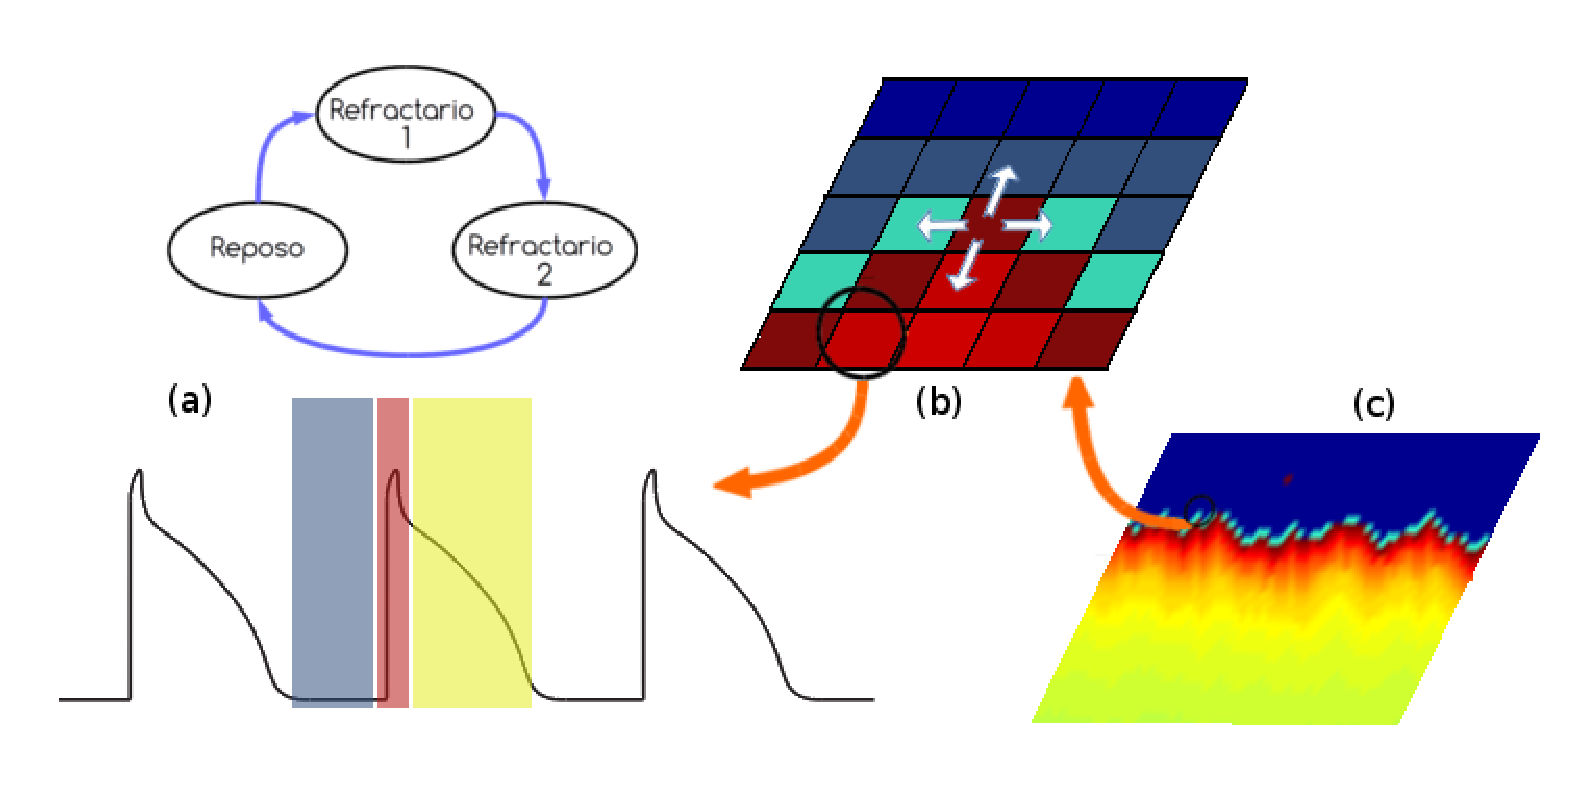
\epsfig{file = ./images/01_chap/automata1.eps,width = 14cm}
% \caption{Represetación del módelo del autómata celular. (a)Prototipo de \ac{AP}
% con niveles de $V_m$. el nivel de $V_m$ se asocia a los tres estados del
% automata definidos en \cite{Alonso-Atienza05} (b) Cada celda esta modelada por
% medio del autómata celular, que se conecta con 4 vecinos, la vecinda  tiene
% forma de cruz  y esta commpuesta por 5 celdas. (c) representación de la propagación
% del \ac{AP} en un tejido de 100x100 celdas.}
%   \label{fig:automata1}
% \end{figure}
%
% En la propagación del \ac{AP}, la despolarización de la célula, en el modelo
% \cite{Alonso-Atienza05}, se define en terminos probabilísticos y , se tienen en
% cuenta el grado de excitabilidad de la célula (E) y la cantidad de celdas
% exitadas de la vecindad (Q). Por lo tanto, si ${P_{j}}^{exc}$ es la
% probabilidad de excitación de la célula, decimos:
%
% \begin{equation}\label{eq:Propaga}
% P_j^{exc}= k\cdot E\cdot Q
% \end{equation}
%
% Donde $k$, es una constante de proporcionalidad. $E$ viene determinda por las
% curvas de restitución de \ac{CV} y $Q$ es definida en función del número de
% células que se encuentran en estado Refractario 1. Por lo tanto, al aumentar
% \ac{CV} la ${P_{j}}^{exc}$ de la célula $i$ aumente, y de igual manera, sucede
% si se aumenta el número de células vecinas recien estimuladas.
%
% Cada célula en el automa celular tiene la capacidad de excitar a las
% células vecinas sólo cuando dicha célula se encuentra en el estado
% Refractario 1. Se codifican los estados de la célula en (A):
% 1 cuando la célula esta en estado refractario 1 y, 0 si la
% célula ha perdido la propiedad de excitar a otras células
% \cite{Alonso-Atienza05}, por lo tanto, $P_j^{exc}$ esta definida por:
%
%
% \begin{equation}\label{eq:Propaga2}
% P_j^{exc}= k \cdot E\cdot\sum_{i \neq j}\frac{A_i}{d_{ji}^2}
% \end{equation}
%
% Donde $i$ indica una celda pertenecientes a la vecindad de la célula $j$. $A_i$,
% representa la codificación de los dos estados de la célula, (1 o 0) y $d_{ji}$
% es la distancia de conexión entre la celda $i$ y la celda $j$.
%
%
% Aca seria bueno poner como se generan las dinamicas variando cv y apd, eso lo
% tengo yo ahi en el computador de la sun,,, de esta forma validamos el uso de
% este automata para la tesis
%
% Por lo tanto, se puede hablar que el módelo del muúculo cardiaco, a través de
% \ac{AC}, es una simplificación del tejido cardiaco, que permite  simular las
% propiedades de propagacion del \ac{AP}.
%

\subsubsection{módelo de reaccion-difusión}

% Los módelos reaccion-difusión para representa la dináica del tejido cardiaco,
% por un lado modelan la conexión  entre las células a partir de
% resistencias eléctricas y, por otro lado la actividad eléctrica de la célula es
% reproducica con la simulación de los canales  y corrientes iónicas. A primera
% instancia se observa que este tipo de modélo es mucho mas realistas y por lo
% tanto, la dinamicas cardiacas complejas son reproducidas de mejor manera.
%
% Los sistemas de reacción-difusión, utilizan ecuaciones diferenciales no lineales
% para describir el proceso de excitación de la celular y propagación.
%
% \begin{equation}\label{eq:r-d}
% \frac{\partial{u_i}}{\partial{t}}=f_i(u_i, \ldots,u_n) + \nabla \dot
% (\mathbf{D}_i \nabla u_i), i=1,\ldots.n
% \end{equation}
%
% Donde $u_i$ es la variable de estado, para el caso del tejido cardiaco $u_i$
% represtna la diferencia de potencial de la transmembrana, la conductividad de
% los canales  y la concentración iónica \cite{Sachse04}. $f_i$ es el grado de excitación, y
% $\mathbf{D}_i$ el tensor de difusión. a su vez el cambio de estado es
% determinado por $f_i$ y $\nabla \dot(\mathbf{D}_i \nabla u_i)$
%
% Para el musculo cardiaco, se considera que el tejido se comporta
% como un sistema compuesto por tres medios continuos \cite{holden1997}, el medio
% intrecelular, el medio extracelular y la membrana celular. lo que conlleva a
% representar las celulas electrofisiológicas con la aproximación de dos modelos
% el modelo bidominio y el modelo momodominio.
%
%
% Estos dos modelos, el bidominio  y monodominio, combinan los
% modelos electrofisiológios, con el flujo de corriente a través de los espacios
% extracelulares y/o intracelulares, respectivamtente. Como se observa en la
% figura \ref{fig:mono_bidominio}, este enfoque biofisico, une el modelo de
% menbrana celular con el modelo de corrientes, este último modela el acoplamiento
% eléctrico de la conductividad de membrana celular con el medio, a través de
% resistencias. La diferencia de los modelos bidominos y monodominos, es por lo
% tanto, el número de dominos que maneja el modelo, para el flujo de la corriente
% eléctrica.
%
% \begin{figure}
% \centering
%  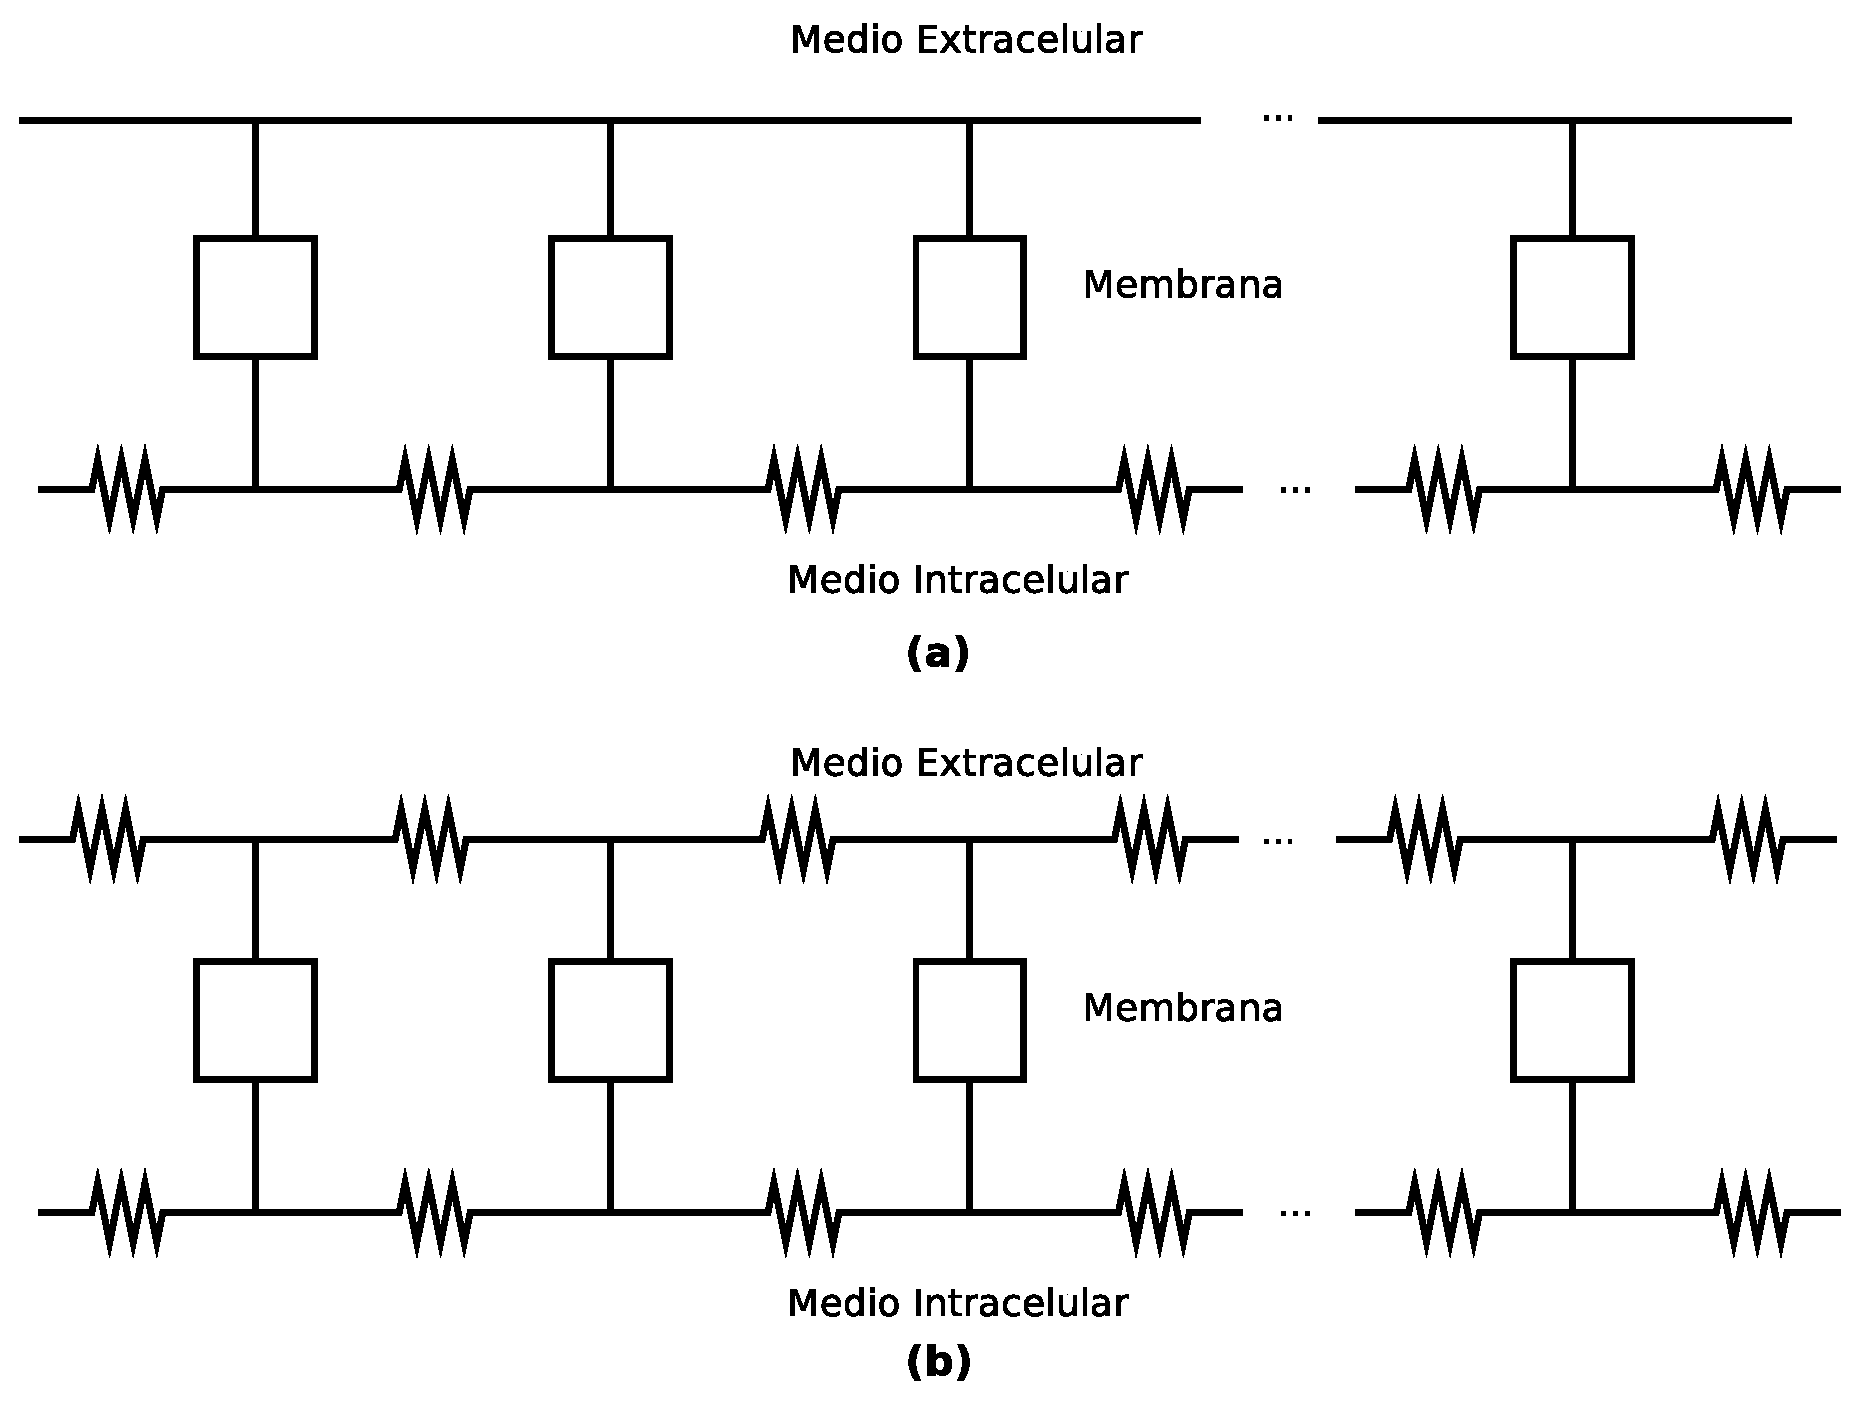
\epsfig{file = ./images/01_chap/modelosbiofisicos.eps,width = 14cm}
% \caption{Diagrama del modelo de tejido unidimensional simulado. Modelos
% circuitales biofísicos: (a) monodomino y (b) bidominio}
%   \label{fig:mono_bidominio}
% \end{figure}
%
%
% El modelo monodominio incorpora los efectos de la conductancia
% intracelular, y asume que la diferencia de potencial entre el medio extracelular  y la
% menbrana es cero. en otras palabras el potencial de membrana $V_m$, es equivalente al
% potencia intracelual $\theta_i$.
%
%
% En el modelo bidominio \cite{henriquez1992, miller1978}, el tejido cardiaco está
% compuesto por dos medios continuos, uno intracelular y otro extracelular que ocupan el
% mismo espacio físico. el medio intracelular representa el interior de la célula,
% mientras que el medio extracelular modela el espacio entre célular. se habla de
% que los espacion son continuosm en el sentido  que las corrientes pueden fluir
% de una célula a otra, a través del medio intracelular (debido a las uniones
% comunicantes), sin tener que pasar por el medio extracelular.
%
%
%
%

\section{Sistemas de medida}


% http://www.bem.fi/book/
%
% Como se ha visto, las fuentes cardiacas son procesos bioeléctricos que se generan
% durante la contracción del corazón. En otras palabras, el paso de corriente a través de la
% membrana de las células que estan exitadas. Por lo tanto, la actividad de las fuentes
% cardiacas pueden ser modeladas matematicamente como fibras cilíndricas simples, y se puede describir
% como fuentes electricas del tipo monopolos o dipolos  \cite{Malmivuo95}.
%
%
%
% A lo largo de esta Tesis, se modela las fuentes cardiacas como la variación
%
%
%
%
% The excitation propagation process can be registered with extracorporal
% electrodes
%
% In this study, we model cardiac sources as a
% time-varying dipole field, i.e. as a spatial distribution of time-varying
% dipoles $\mathbf{J}(v,t)= [J_x(v,t), J_y(v,t), J_z(v,t)]^T$ on a volume $V$,
% where $v$ denotes a point located inside $V$ and $t$ denotes the time instant.
%
%  The time-varying activity of cardiac sources can be measured by lead systems,
%  producing cardiac signals. Taking the dipole field as our reference description
%  for cardiac sources, we follow a lead-field approach to model cardiac signals
%  \cite{Malmivuo95}. According to the lead-field theory, the cardiac signal
%  $c(t)$ that is induced at a lead system by a dipole field $\mathbf{J}(v,t)$ can
%  be expressed as
%
% \begin{equation}\label{eq:EqSintesis}
% c(t)=\int_V{\mathbf{L}^{T}(v) \mathbf{J}(v,t)}{dv}
% \end{equation}
%
%  where the vector field $\mathbf{L}(v)= [L_x(v), L_y(v), L_z(v)]^T$ is the
%  measurement sensitivity distribution (MSD) and describes the ability of the
% l ead system to measure cardiac dipoles located at $v\in V$. In words, cardiac
% si gnals are a weighted linear combination of the underlying cardiac sources.
%
%
%
\subsection{Sistema de Electrodos}
% definición de las ecuaciones lapalaciano
% \subsection{Volumen equivalente de sistema de electrodos}
%  \ac{LF}


\section{Conclusiones}
